\documentclass[12pt,a4paper]{article}
\usepackage[utf8]{inputenc}
\usepackage[T1]{fontenc}
\usepackage{amsmath}
\usepackage{textcomp}

\usepackage{geometry}
\geometry{a4paper,left=25mm,right=25mm, top=2cm, bottom=2cm} 

\usepackage{graphicx} %fuer bilder

\usepackage{verbatim}




 \usepackage{mathptmx}
 \usepackage[scaled=.90]{helvet}
 \usepackage{courier}



\usepackage{listings}
\usepackage{color}
 
\definecolor{dkgreen}{rgb}{0,0.6,0}
\definecolor{gray}{rgb}{0.5,0.5,0.5}
\definecolor{mauve}{rgb}{0.58,0,0.82}

\pagestyle{empty}
\lstset{numbers=left, language=VHDL}
\lstset{showstringspaces=false,
basicstyle=\ttfamily\footnotesize,
breaklines=true,
tabsize=3,
commentstyle=\color{dkgreen},      % comment style
inputencoding={ansinew},
title=\lstname %zeigt titel der datei an
}

\usepackage{pdfpages} % fuer pdfs
\usepackage{hyperref} % fuer url


%keine einrückungen bei absatz
\parindent 0pt

\begin{document}
\title{Übung 02}
\author{Reinhard Penn, Bernhard Selymes, Robert Zeugswetter}
\date{November 2015}

\normalsize


%Beginn des Dokuments

\newcommand{\Uebung}{ScanChainInsertion}
\newcommand{\srcpath}{../../src}
\newcommand{\simpath}{../../sim}
\newcommand{\synpath}{../../syn}

%Angabe
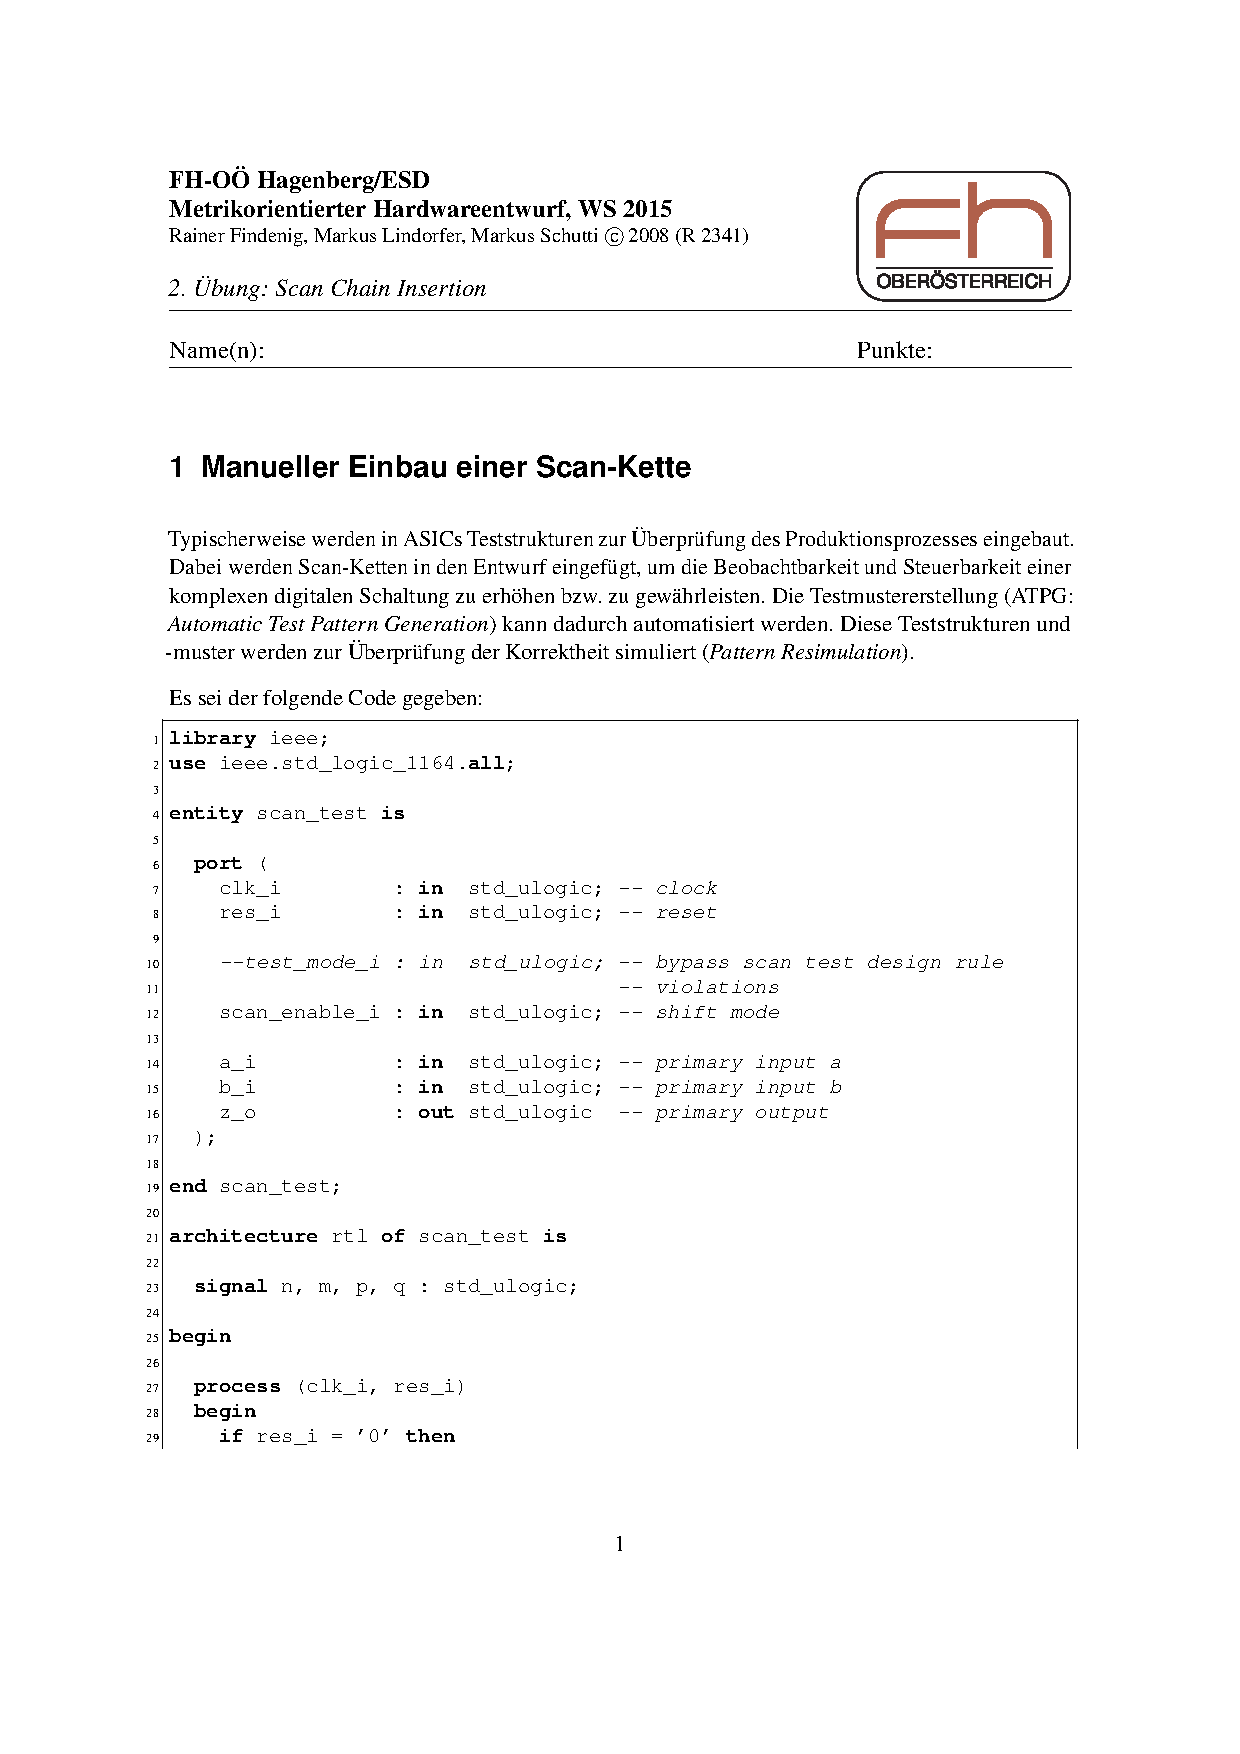
\includepdf[pages=-]{../Angabe.pdf}

\begin{center}
Scan Chain Insertion\\
Übungsprotokoll zur Übung 2\\
Metrikorientierter Hardwareentwurf\\
Bernhard Selymes, Reinhard Penn, Robert Zeugswetter\\
24.11.2015
\end{center}


\section{Manueller Einbau einer Scan-Kette}
Als Flipflops werden DFSC1 und DFSC3 verwendet, da diese die Pendants zu DFC1 und DFC3 sind.\\
Es ist sinnvoll nicht belegte Ausgänge der Flipflops zu verwenden, da sich dadurch die Treiberstärke aufteilt.

\subsection{Erstellen des Testmusters}
\begin{verbatim}
a)
n m p q
1 0 0 0

b)
q = 0
	p = !q
	1 = !0

b_i = 1
	p = ((a_i xor b_i) and b_i) or !(a_i xor b_i)
	
	bei a_i = 0
		((0 xor 1) and 1) or !(0 xor 1) = 1 or !0 = 1
		
	bei a_i = 1
		((1 xor 1) and 1) or !(1 xor 1) = 0 or !0 = 1
\end{verbatim}

\section{Source Code}
\subsection{Manuelle ScanChain}
\lstinputlisting[linerange=32-55, firstnumber=32]{\synpath/netlist/scan_test_mod.vhd}

\subsection{Manuelle ScanChain mit Fehler}
\lstinputlisting[linerange=32-57, firstnumber=32]{\synpath/netlist/scan_test_mod_fail.vhd}

\subsection{Testbench}
\lstinputlisting[linerange=32-57, firstnumber=32]{\srcpath/scan_test_tb.vhd}

\section{Simulation}

\begin{figure}[ht]
\centering
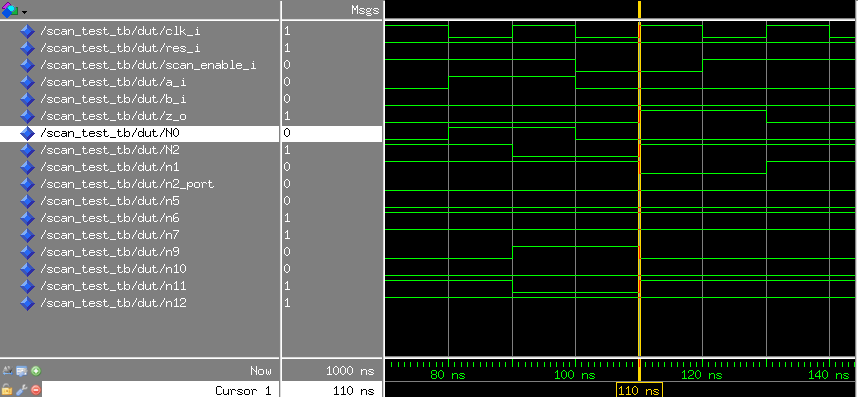
\includegraphics[width=\textwidth]{wave}
\caption{Waveform von Simulation ohne Fehler.}
\end{figure}

\begin{figure}[ht]
\centering
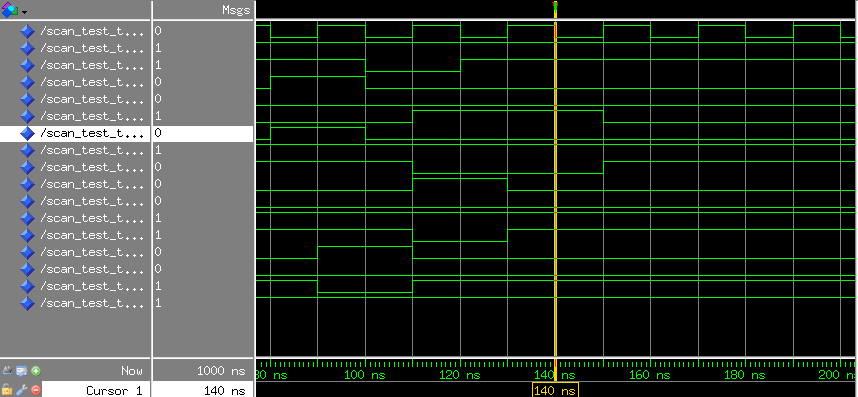
\includegraphics[width=\textwidth]{wave_fail}
\caption{Waveform von Simulation mit Produktionsfehler. Assertion löst aus.}
\end{figure}

\section{DfT-Verletzungen}

\subsection{No asynchronous design style}

\subsection{No on-chip generation of clock signals}

\subsection{Special attention when more clock domains}

\subsection{No gating of clock signals}

\subsection{No combinatorial feedback loops}

\subsection{No one-shot delays}

\subsection{No on-chip generation of asynchronous control signals}

\subsection{Avoid tristate signals, check for bus contention}

\end{document}
